\chapter{Managing software deployment in distributed systems}
\label{ch:managingDS}
In the previous chapter we addressed the issues raised while managing the software layer of complex distributed systems, and more specifically Internet of Things systems.
For instance, classical information systems are nowadays a critical piece of many important processes as well as industrial than commercial.
Downtime of this systems can represent a big economic loss, therefore robustness and continuous availability should be assured.
Thus, the evolution of the needs and the rapid obsolescence of features imposes an openness to new functionalities that were not predictable at design time.
In IoT systems, we can take the example given in subsection \ref{subsec:effBuilding}, in which evolutions of a building were complicated to predict.
It was even more difficult to provide a prepared software platform able to deal with new features and devices, preventing a managed deployment of new services.
However, this new behavior must be implemented in the future due to the new energy policies, without alter the current given services.

In this chapter I will first present the general concepts of deployment, which can be diverse according to the different perspectives of software life cycle.
For this thesis, I will give my own definition of software deployment, which covers from the availability of a binary file ready to be executed, to the distribution, dynamic loading and linking on a running platform, either as a new feature or to perform an update.
Indeed, software deployment is not a new problem, but as shown in the previous chapter, the architectures where we try to apply the typical approaches have evolved, from centralized systems to large-scale distributed systems with resource-constrained nodes.
In this context, deployment for monolithic, homogeneous targets will be described, followed by its main principles for distributed, non-monolithic and heterogeneous systems, leveraging software engineering approaches.
The aim is to provide a general understanding of the issues already covered by software engineering, which are also present in IoT systems.
Once these issues are presented, a focus on distributed systems deployment will be performed, in order to make a fine comparison on the deployment methods and its potential application to IoT systems.
A state of the art of the deployment methods specially conceived for IoT devices is then discussed, finishing by a conclusion.

\section{Overview}
As we discussed in the previous chapter, we can compare classical distributed systems with IoT systems.
Since they share both the high number of participating nodes and the collaborative approach to offer services, the existing proposed solutions to manage the software layer in classical distributed systems are of high interest, and provide a good insight for their adoption in the IoT.
A definition of a distributed system proposed by Coulouris \textit{et al.} can be found at \cite{coulouris2005distributed}:
\begin{citeverbatim}
	" We define a distributed system as one in which hardware or software components located at networked computers communicate and coordinate their actions only by passing messages."
\end{citeverbatim}
With this definition, we can clearly realize an IoT system that fit this characteristics, being an IoT device a computing machine which is part of a network including other IoT devices.
Thus, the challenges arose by classical distributed systems will be the same for the IoT based systems.
Taking this into account, it is possible to explore existing solutions that are most adapted to IoT systems, regarding the main differences stated in the synthesis of the previous chapter.

First, the high acceptance of Component Based Software Engineering (CBSE)\cite{crnkovic2002building} approaches to deal with the large size of a software architecture lead our investigations to explore it for its potential use in the IoT, in order to reliably manage the life cycle of these large information systems.

Second, as the system evolves, new dynamic deployments will be required to offer adapted functionalities.
This is challenging in single software deployments, and even more in a distributed environment.
Kramer and Magee\cite{kramer1990evolving} provided, albeit in an informal way, in their article that introduces quiescence, a definition for what we consider to be dynamic evolution:
\begin{citeverbatim}
	" [Evolutionary change] may involve modifications or extensions to the system which were not envisaged at design time.
	Furthermore, in many application domains there is a requirement that the system accommodate such change dynamically, without stopping or disturbing the operation of those parts of the system unaffected by the change. "
\end{citeverbatim}
This kind of evolutions will be systematically present in IoT systems, as we stated for instance in the case of building automation in section \ref{subsec:effBuilding}.

Thus, the use of CBSE approaches to support such evolutions is worth considering, since decoupling the large distributed system into small components results in an easier software life-cycle management.
However, managing the deployment of these components is a known issue, which becomes more important when we take into account the constraints typical of IoT devices.

\section{Software deployment}
\label{sec:softDeployment}
%In software engineering, software development issues were addressed in several %ways, in order to hide the inherent complexity of integration, deployment and management of software systems.
%One important advancement on this is the use of \textit{Middlewares}, which stand between the OS and the applications.
%Its main properties are based on hiding certain complexities such as network details for distributed systems or simply the overall application development.
%The evolution of these middlewares have come to hide heterogeneity, mobility, data processing and scalability, in the form of blocks, easier to maintain.
%Several software engineering principles such as separation of concerns and modularity have been adopted by middlewares, to manage the increasing complexity of applications and to ease programmability.
%Moreover, runtime support for managing applications during their execution are proposed by recent works in this domain\cite{mikalsen2006putting}.
As software complexity has increased over the years from old computing systems managed only by experts to today's personal computers managed by end users, new methods for software development and deployment appeared.
The need of reliable, robust, and fixed production cost of software motivated various research fields on software engineering, which helped to build large projects fulfilling such characteristics.
Several tools were developed to facilitate software production during the life cycle of the applications.
Approaches from software engineering have been developed and improved, such as code complexity analysis, testing tools, shared libraries, code interpreters, requirement analysis tools, compilers, dependency management tools, deployment and monitoring tools, and so forth.

In order to give a better understanding of an application's life cycle, we can divide the previously mentioned tools into three families, which aim to ease the conception and execution of such applications:
\begin{itemize}
	\item \textbf{Development tools.} While creating an application, development tools such as \textbf{programming languages, compilers} and \textbf{debuggers} are used. 
	On the project's infrastructure side, tools facilitating collaboration between development teams for construction and maintenance of applications are found, for instance: \textbf{code analysis tools, bug tracking and issue management, version control, product engines and project management tools.}
	\item \textbf{Runtime tools.} With the emergence of distributed computing, \textit{middlewares} appeared to cope with the problem of interoperability between networked machines.
	This was caused by the use of different communication protocols.
	An intermediate layer that abstracts the differences in architecture and protocols was put in place, to be used as a translator.
	Moreover, middlewares are also used to provide other functionalities, such as \textbf{runtime management, data persistence} or \textbf{monitoring} of applications.
	\item \textbf{Management tools.} In large-scale computing systems, such as distributed and IoT environments, management helps system administrators and operations teams to have control on the supervision and installation of applications.
	The management domain can be divided into three categories: \textbf{deployment, monitoring} and \textbf{administration.}
	The deployment process involves the sequence of actions that brings software from development to execution, while ensuring the adaptability of the software according to the changes in the context.
	Monitoring is needed to follow the evolutions of the system, in order to find problems on software or hardware.
	\item \textbf{Administration tools.} Finally, administration encompass the configuration of hardware and low-level software stack, mainly dealing with the continuous growth of types of actions and configurations when using multiple machines for distributed applications.
\end{itemize}

The focus of this work is to propose IoT solutions based on three tools: runtime, management and administration.
% while development tools will be covered in future work.
More specifically, a management tool is proposed to deal with the deployment issues typical of IoT systems, leveraging software engineering existing approaches to solve very similar issues.
Thus, deployment must be defined in our context, in order to study the typical approaches with a focus on distributed environments.
Discussion of this topic is carried through the next section.

\subsection{Deployment definitions}
In the last years, software deployment has suffered several changes in its execution environment.
As today, it is not a "one-time" process, but rather an iterative operation for the sake of improvement and continuous evolution.
As a result, consecutive cycles of software re-design, development and maintenance are carried through the lifespan of an application.
To formalize this evolutions and the process itself, several definitions of software deployment have been proposed, every one empathizing different aspects.
In the context of component-based systems, Szypersky\cite{szyperski2003component} define it as follows:
\begin{citeverbatim}
	" Deployment is the process of readying such a component for installation in a specific environment. 
	The degrees of deployment freedom are typically captured in deployment descriptors, where deployment corresponds to filling in parameters of a deployment descriptor. "
\end{citeverbatim}
This definition highlight the use of components as a form of deployment, based on the concept of \textit{descriptor}.
Moreover, it describes the process as the installation and configuration of these components in an environment.
Another definition coming from the Object Management Group Deployment and Configuration of Component-based Distributed Applications Specification (OMG D+C) is broadly used as a reference.
In the specification \cite{specification2006deployment}, it states the following:
\begin{citeverbatim}
	" Deployment is defined as the processes between acquisition of software and its execution. [...] In order to instantiate, or deploy, a component-based application, instances of each subcomponent must first be created, then interconnected and configured. "
\end{citeverbatim}
A more general definition was proposed by Carzaniga in \cite{carzaniga1997characterization}:
\begin{citeverbatim}
	" Informally, the term software deployment refers to all the activities that make a software system available for use. [...] The delivery, assembly and management at a site of the resources is necessary to use a version of a software system. "
\end{citeverbatim}
We can find in this definition the notion of \textit{assembly, delivery} and \textit{management}, as well as an emphasis on a site where those activities are applied.
Details of these activities are given by Hall \textit{et al.}\cite{hall1999cooperative} in our last definition:
\begin{citeverbatim}
	" Software deployment is actually a collection of interrelated activities that form the software deployment life cycle. 
	The software deployment life cycle, as we have defined it, is an evolving definition that consists of the following processes: release, retire, install, activate, deactivate, reconfigure, update, adapt, and remove. "
\end{citeverbatim}

The cited definitions are a good guidance to establish a more complete and proper definition in our context of an IoT environment.
The process of deployment is described as a development of a software product until its distribution and execution.
Throughout this process the life cycle of the system is performed.
In the case of IoT systems, the process can be the same, although the methods are very different.
Componentization, distribution and installation of an IoT application have platform-specific constraints which avoid a generalization of the process.

In order to take into account these constraints, a definition of software deployment in IoT environments can be proposed as:
\begin{citeverbatim}
	" The process between the production and execution of platform-dependent software systems, following similar activities as in classical deployment consisting in making configurations and bringing the software to its desired execution state. The process can continue along the lifetime of the software system in order to bring it to a new state via reconfigurations and updates, which are subject to the platform resources constraints. "
\end{citeverbatim}
It is then necessary to deal with these platform-specific constraints, using abstractions such as component-based development and deployment management, which are already proposed by software engineering tools for classical distributed systems.
Indeed, decoupling IoT environments into software components and manage their deployment is not an easy task, since memory constraints, processing power, energy autonomy and network topology prevents the direct implementation of the same approaches, being one of the motivations to conduct this research.
Basic concepts of Software Engineering abstractions are necessary, in order to adapt them for meeting these constraints.
Such concepts will be described in the next sections.

\subsection{Deployment of monolithic, homogeneous systems}
\label{subsec:singleDeployment}
As the cycle of software development, release and delivery speed increase very quickly, automation of these processes are needed.
One of the most common deployment process is the one which is carried in single machines.
In this case, deployment is performed without any issues of heterogeneity, planning, and coordination, present in typical distributed systems, and inherently in the IoT.
Thus, automate this process results in a less challenging task.
However, it is important to study these approaches as a foundational effort for deployment automation in general.
We can divide these technologies into three main principles:
\begin{itemize}
	\item \textbf{Package managers.} Mainly used in Linux and UNIX-like OSs, these tools have as goal the deployment of software previously packaged in a standard format. 
	RPM package manager and dpkg are examples of standard package managers.
	In order to manage multiple packages, usually required as dependencies, an application can be modeled as a graph of interdependent packages.
	High level tools such as Yellowdog Updater Modified (YUM) and Advanced Packaging Tool(APT) are used to automate the deployment process, which consists in retrieving, installing, updating and uninstalling applications, by calculating the tree of dependencies.
	\item \textbf{Application installers.} They are based on an application-centric deployment model, in contrast to package managers which are based on dependencies.
	Windows Installer and InstallShield are examples of tools using this approach, on the basis of features and components.
	Features are the functionalities that can be or not installed according to the user, and components are the parts to compose such features.
	The composing mechanisms such as the needed components and the order to install features, which are hidden to the user, are determined from the installer.
	\item \textbf{Web-centric deployers.} In order to transfer software in a controlled, secured way, web-centric deployers appeared with the growth of the Internet.
	The purpose of this approach is to transfer executable software artifacts from a remote (web) server to an end-user's computer.
	With a view to secure the application deployment due to the web-based approach, only trusted applications can run within a protective environment, which is well isolated from the local resources.
	Implementations of this method are, for instance, Java Applets, ActiveX components, Java Web Start (a reference implementation of Java Network Launching Protocol (JNLP) standard), .Net ClickOnce and ZeroInstall.
\end{itemize}
As we can see from the above principles of deployment, the high dependency of the execution environment forces the development of automated tools targeting only a certain platform.
However, making some abstractions from the platform such as web-centric and Virtual Machine (VM) execution environments, it is possible to deploy artifacts independently of the running OS.
As for the IoT, since there are no widely used OS or execution environments for IoT devices, it is very complicated to develop automatic deployment methods using the same abstractions.
Moreover, the use of high level execution environments such as VMs it is not worth considering, due to the scarce resources found on this devices.
Nevertheless, it is clear that the component-based approach appears in the three presented methods, thus we will explore this approach and leverage its main principles to propose a proper implementation for IoT devices.
The next section will present the Component Based Software Engineering, followed by its common implementations.


\subsection{Component Based Software Engineering (CBSE)}
\label{sec:CBSE}
Several definitions to CBSE have been proposed in the literature, being the notion of \textit{component} the main principle.
In a general way, CBSE aims to leverage the main benefits of SE in terms of development, integration, maintenance, reusability, separation of concerns, among others.
However, a more specific definition was proposed by Szyperski\cite{szyperski2002component}, being one of the most used:
\begin{citeverbatim}
	" A software component is a unit of composition with contractually specified interfaces and explicit context dependencies only. A software component can be deployed independently and is subject to composition by third parties. "
\end{citeverbatim}
In another definition, Heineman \textit{et al.}\cite{heineman2001cbse} define a component as:
\begin{citeverbatim}
	" A component model defines a set of standards for component implementation, naming interoperability, customization, composition, evolution and deployment. "
\end{citeverbatim}
We can note that this definition puts more emphasis in the development model, which not only leverages the abstract system composition, but also covers the global system deployment from the underlying pieces.

The main characteristics of a component can be summarized as follows:
\begin{itemize}
	\item \textbf{Interfaces specification.} The available functionalities of a component.
	\item \textbf{Explicit dependencies.} A component could require other component's functionalities or native libraries to work correctly.
	If so, such requirements should be exposed.
	\item \textbf{Instantiation.} Multiple instances of the given type can exist.
	\item \textbf{Deployment independence.} A deploy unit represent the whole component, which can be reused. However, this feature can be discussed.
\end{itemize}
Moreover, a component-based approach can define an \textit{Architecture Description Language (ADL)}.
This is useful to describe the structure of a software, in a formal way\cite{taylor2009architectural}\cite{len2003software}\cite{medvidovic2000classification}.
ADLs are declarative languages that describe a system's architecture as a set of components, connectors, bindings and configurations.
Such a language can be used to assemble components, based in two elements:

\begin{itemize}
	\item \textbf{Instances.} They are the main elements which actually embody the required application's functionalities, constituting the business logic.
	\item \textbf{Connectors.} A link between component's instances, determined by the exposed provided and required functionalities of the used types.
\end{itemize}

In an ADL, the specified interfaces can be bound between component instances through connectors, which are identified as "required" and "provided" interfaces.
The complexity management can be achieved using a descriptive hierarchical composition, allowing scalability.
For instance, Fractal\cite{bruneton2006fractal} provides a structural description of software architecture.
However, the needs can differ between systems, in order to associate functional, behavioral and system properties with the architecture.

The division in small pieces of a big architecture such as the IoT software layer, can be very useful from a development and maintenance point of view, leveraging the component decoupling and the use of bindings between components to providing services.
Indeed, an ADL can ease the task of composing such layer, giving a complete management of the component's life cycle, from the deployment to the instantiation, being one of the main concerns of this thesis.
Moreover, we can associate to the defined characteristics of components and its composition to an execution environment, which is in charge of the exploitation.
However, the component's implementation is not defined at this level.
The next section will describe some of the most common resources used to achieve deployment of component-based applications.

\subsection{Resources for CBSE based deployment}
The deployment facilities already introduced in section \ref{subsec:singleDeployment} are intended for deploying traditional applications.
The necessary deployment information is managed by these deployment systems, such as dependencies, geographical distribution on target sites, availability of required resources on these sites etc.
Programming of component-based software follows modular design principles, providing a broader view of the system.
The objective is to predict the deployment state during development, which is facilitated using component-based programming.
Moreover, the models present in component execution platforms provide explicit means to describe components and their dependencies.
Three important execution platforms are presented in this section, in which a modular development is used in order to fit the execution environment that host the components.
Descriptions of these platforms are based on how the components are described and packaged, how does the deployment descriptor of those is created and in which ways these platforms addressed previously introduced issues.

\begin{itemize}
	\item \textbf{CORBA Component model.}
	CORBA (Common Object Request Broker Architecture) was defined by the OMG as a standard to provide an execution platform which enables the development of components in several computer languages, while it can be executed on multiple computers to work together.
	The execution platform for distributed CORBA based software is called Corba Component Model (CCM)\footnote{\url{http://www.omg.org/spec/CCM/4.0}}, in which a component is defined by an interface and one or more implementations of that interface.
	A CORBA deploy unit is packaged in a zip format, which contains the description of the component files, the implementation binaries and a file to express the properties.
	A set of logical interconnection of components forms a CCM components assembly, which is distributed over various machines.
	The connections between components are done during the deployment phase, in which the assembly will be physically installed on a given configuration of machines.
	A descriptor file in the form of a \textit{.cad} (Component Assembly Descriptor) file is used by the CCM, which contains the description of the assembly handle and a set of component packages, containing the components involved in the assembly.
	The CORBA runtime is in charge of the deployment activities, including transfer, installation, composition, instantiation and configuration of components on targeted runtimes.
	%The deployment process is specified by the CCM with a number of steps to be carried during the process, which consists in the definition and selection of deployment sites, installation of implementations using the information contained in the descriptor software package, instantiation of components and finally connection of components.
	
	\item \textbf{EJB.}
	For the construction of enterprise Java applications, an API was specified by Sun Microsystems\footnote{\url{http://download.oracle.com/otndocs/jcp/ejb-3_0-fr-eval-oth-JSpec/}} which describes a managed, server-side component architecture called Enterprise JavaBeans (EJB).
	In EJB a standard way to implement business code usually found in enterprise applications is provided.
	The addressed problems in such code are handled by EJB, including persistence, transactional integrity, and security, which are handled in a standard way, avoiding the re-implementation of this often repeated concerns.
	Thus, the programmers are free to concentrate on the particular problem at hand.
	
	The EJB specification also includes a definition for installation, activation, deactivation and uninstall beans.
	In contrast to what could be expected, the deployment of applications based on beans are defined in an archive file, instead of using the bean as deploy unit.
	An XML file act as deployment descriptor, contained in the archive file.
	Typically, information about transactions, security and persistence required for each bean is present in the descriptor.
	One of the main elements defined by the EJB specification for deploy units are the archive format and content of the deployment descriptor.
	Coordinated deployment of beans on distributed systems is not addressed in the EJB specification.

	\item \textbf{OSGi.} Closely related to the IoT, OSGi (Open Service Gateway initiative) was originally created to provide a general component model for Java platforms, running on top of domotic residential gateways.
	This model aims to implement a dynamic module deployment based in \textit{Bundles}.
	The OSGi specification defines a life-cycle manager of this bundles, which are a set of encapsulated components.
	A Bundle designates a specific package from a JAR, which is mandatory for the deployment.
	Dependency contracts can be declared using manifest files, leveraging the notion of Java packages pointing to other bundles or parts of them.
	An \textit{Activator} class represents the internal code of a component, which defines the life-cycle of the Java module including code to start and stop the application.
	Moreover, the OSGi framework defines the Java modules that can be deployed at runtime whose granularity dependency is represented using either the JAR or the Java package of the Activator class.
	This framework also defines the notion of internal service, using a central services registry already defined in the previous section, allowing dynamic inscription of new services.
	Thus, OSGi component contracts are dependency oriented.
	Two main implementations of this framework are Apache Felix and Eclipse Equinox, being the first used in several Enterprise Service Bus and the latter the architecture of the Eclipse development environment.
	
	A project called OpenTheBox\footnote{\url{http://openthebox.org/}} is the result of a OSGi platform implementation dedicated to domotics.
	It is based on the OSGi platform Knopflerfish\footnote{\url{http://www.knopflerfish.org/}}.
	The core of this project relies in a central manager called Apam\cite{damou2013apam} running in the home automation box, which provides an isolated collaboration environment between applications\cite{estublier2012managing} and controls the conflicting accesses to the shared devices\cite{estublier2013resource}.
	
	The specification allows interactions anticipated by the services architecture, but they must be managed manually by the developer.
	This task is very delicate and requires a deep knowledge of the OSGi mechanisms in order to finely handle all the possible cases to avoid errors.

%A new technology is then necessary to manage automatically all this interactions, proposing a solution to the manual management of them.
%This technology, called iPOJO, is described in the next subsection.

%\subsubsection{iPOJO}
%Apache iPOJO (injected Plain Old Java Object)\cite{escoffier2007ipojo}\cite{escoffier2007dynamically} is an implementation of the service-oriented components approach.
%It was developed at Grenoble Informatics Laboratory (LIG in French), at Ad\`ele team.
%It relies in the Apache Felix\footnote{\url{http://felix.apache.org/site/index.html}} OSGi open-source implementation.

%As stated in the previous subsection, an easy-to-use approach to develop applications in top of OSGi is required.
%In this point of view iPOJO aims to simplify the development of dynamic services applications, implementing service-oriented components already described previously.
%This platform is based on the OSGi specification, and consequently, it inherits its characteristics: dynamic, centralized and with Java support only.

%The iPOJO technology offers:
%\begin{itemize}
%	\item \textbf{A model strongly coupled with an execution machine.} In order to give a more comprehensible application structure, all the components of the model exists at execution time.
%	\item \textbf{An isolated dynamic service architecture.} Beyond the dynamic service architecture interactions derived from the OSGi platform, an isolation principle is also proposed, providing some services with private characteristics.
%	\item \textbf{A simple development model.} The iPOJO execution machine provides introspection injection allowing a transparent management of this concerns to the developer. 
%	Thus, the SOA complexity is hidden using the development model from Plain Old Java Object\cite{fowler2000pojo} concealing specially the complexity of the OSGi dynamism.
%	\item \textbf{A structural composition language.} iPOJO allows application building from a structured service composition.
%	The composition is modeled with the services' specifications, regardless of the implementation.
%	This decoupling is one of the iPOJO advantages, since this way the infrastructure choices at runtime an available implementation.
%	Therefore, the applications conceived using this method are managed dynamically.
%	\item \textbf{Dynamic reconfiguration and introspection functionalities.} This offers a reflected overview of the system structure changes due to dynamism.
%	\item \textbf{Extensibility mechanisms.} New non-functional properties can be easily added, such as persistence, security or quality of service.
%\end{itemize}

%iPOJO leverages this mechanisms to allow a simpler construction of dynamic service applications, while respecting the dynamic services architecture.
%An important advantage for the developer is the possibility of manage only the desired non-functional properties.
%An application called iCASA\cite{lalanda2014icasa} based on this technologies was created in order to cope with the dynamism of systems such as smart homes.
%Being a part of the IoT infrastructure described in this thesis, it is interesting how a service-oriented component architecture can actually manage the dynamic nature of this environments.
%However, the highly centralized approach, among with the high specialized tools (even if some simplifications are provided), results in a still complex development model.

	A more flexible approach to build component-based applications is introduced afterwards.
	Indeed, providing more flexibility in the implementation language, execution environment and architecture definition would lead to a less complex development model.

	\item \textbf{Fractal}.	Being a generic, yet extensible, component-based model, Fractal\cite{bruneton2006fractal} is one of the most used component-model approach in the research domain.
	It is built as a reflective and hierarchical component model which is mostly intended for its application in deployment and management of software systems such as OS and middlewares.
	Thus, we can find in Fractal the classic concepts of a traditional component model (component, interface, connection) previously described.
	However, the main difference is that it separates a component into two entities:
	\begin{enumerate}
		\item \textbf{Contents.} It contains a finite set of (sub) components and connections.
		\item \textbf{Membrane.} Introspection and manipulation of the components is defined by the membrane, through control interfaces.
		It also defines the connection interfaces to express the required and provided interfaces.
	\end{enumerate}

	Several works\cite{david2005wildcat}\cite{bouchenak2006autonomic}\cite{leclercq2004dream}\cite{romero2010restful} are based on this component model.
	Fractal implementations exists in different programming languages, providing each one additional properties to the model, specific to a particular domain.
	This implementations come from embedded applications supported by the THINK framework\cite{fassino2002think}\cite{polakovic2006building}\cite{hoang2008valentine}, to grid computing using ProActive\cite{caromel2006proactive}.
	Other implementations exists for different languages such as Cecilia\cite{cecilia2015} using the C language, Plasma using C++, Julia\cite{bruneton2006fractal} based in Java, FracTalk in SmallTalk and FracNET in the .NET framework.
	An API is available to control the dynamic evolution of the application, according to which we can create or destroy instances and bindings.
	Even if the hierarchical construction of applications is possible, Fractal does not define a particular mechanism to package and deploy components, since that depends on the chosen implementation.
\end{itemize}

Granted that several CBSE implementations in different languages can be adapted for the IoT, the lack of dynamic deploying mechanisms is a big inconvenient.
Since the goal is to manage a large set of software services using components bound to each other, runtime control on the deployment of new components is mandatory.
Thus, managing software deployment in highly distributed environments, incluing the IoT, should be defined, highlighting the current challenges for non-monolithic, heterogeneous systems software deployment.

\section{Distributed software deployment}
\label{sec:distDeployment}
%\subsection{Challenges in distributed environments}
Distributed systems cannot be managed as centralized systems or single desktop machines, for instance as described in section \ref{subsec:singleDeployment}.
This is due to the very different application domain in which a distributed approach is needed.
Indeed, while desktop applications can be easily deployed through local package and update managers (either at application or OS levels), distributed applications cannot be deployed nor updated using the same methods.
Let's take the example of a set of desktop machines running a typical OS, in which basic functionalities are the same, as well as provided services.
When a new feature is released for such OS, a single binary including the new feature is deployed in all the machines running the OS, regardless of the underlying hardware.
On the other hand, a distributed application cannot be spread among all nodes within the same binary, since each one can offer a different service, or can be in charge of only a part of a bigger system, being the node's hardware capabilities not enough to run such a big application.
This is true for most of the distributed applications, since the goal is to share the resources of several machines (servers) to provide more and better services.
Thus, software complexity can be divided among several machines, deploying different parts of the application in different nodes.
A big challenge appears when it is necessary to deploy new features or update the current ones in this distributed environments, since it is not possible to manually add or update this features for each machine: first due to the quantity and often the physical location of the equipment and second to the uninterrupted use of the application, which cannot be stopped.
The need of a fine management of this software layer is then justified.

Another issue comes with the networking layer availability, which is mandatory for distributed applications.
Since communication is the main activity in a distributed environment, network robustness is then crucial.
However, it is complicated to estimate the network usage for a given application.
As an example, web applications are often exposed to this problem, since they offer their services to an undetermined number of clients.
It is known that as the client requests increase, the application is more susceptible to crash, due to the complex network management of all client's connections.
Usually this problem is solved by deploying more servers in order to increase the number of maximum connections, increasing also the cost of the infrastructure.
In IoT environments this is more complicated, since the number of \textit{things} that are used as servers is limited by the architecture itself, thus the deployment of new things is more complicated.
Moreover, the network robustness found in classical distributed systems is not the same as in IoT systems.
This is due to the network topology already described in the previous chapter.
Even if new protocols to improve this robustness are being developed\cite{thubert2013ietf}, there is always a trade-off between network availability and energy consumption, since most of the communications are done wirelessly by battery powered nodes.
Advancements in more energy efficient transceivers and protocols could improve the communication facilities, giving place to a more flexible usage of the network.

The difficulties presented in this section must be taken into account while developing a solution charged of the distributed applications' deployment.
This solution requires support by some kind of automation tool that should cover as much of deployment activities as possible. 

\section{Deployment on non-monolithic, heterogeneous and distributed systems}
\label{sec:dynamicDeploymentDAS}
An \textit{eternal system} refers to a system which services are required in a constant manner.
Thus, stopping it to make changes such as updates, add new features or other improvements is not allowed.
Such services may include life-critical systems, financial systems, telecommunications, and air traffic control, among many others, including IoT systems which are our concern.
Therefore, techniques are needed to change software while it is running. 
This is a very challenging problem and is known under a variety of terms, such as, but not limited to, runtime evolution, runtime reconfiguration, dynamic adaptation, dynamic upgrading, hot updating, dynamic evolution and so on, sharing the common issue of dynamic deployment.
%In this thesis, we will focus on adapting an IoT architecture and apply those changes at runtime, providing dynamic adaptation through dynamic deployment.

The deployment process usually starts when code is written, or generated, in a programming language, then compiled into binary code to be executed.
Each module of the application is then produced in a form of object file, which a linker can then use to construct a final executable binary or a library (i.e., .dll, .so, .a) if desired.
A symbol table is also embedded with information that defines its dependencies (i.e., shared libraries).
When this code is executed, a process of dynamic linking takes place.
This step is quite different from the previous one, taking into account the information of shared libraries included in the executable file, in order to bind them dynamically to the running process.
A dynamic loader should be provided with the OS, being different one from each other, to offer such functionality.
The same step is performed while updating such a process, with the difference that the previous process must be stopped to be replaced by the new one.
Another approach is proposed for interpreted languages, in which the compilation phase does not take place.
The code in this case is directly executed through an interpreter, which can also use an hybrid approach mixing compilation and interpretation (i.e. Java and .NET).
In this case, the source code is compiled to an intermediate bytecode format, which can be interpreted by a Virtual Machine (VM).
Some optimizations are done in the case of Java, where classes are loaded only when needed.

\begin{figure}[htb]
	\centering
	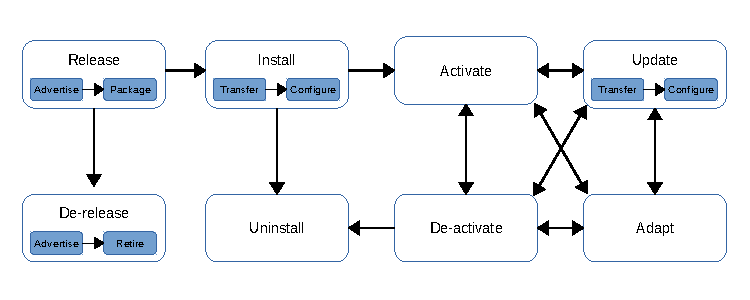
\includegraphics[width=1\columnwidth]{chapters/stateOfTheArt.images/DeploymentActivities.pdf}
	\caption{Software Deployment Activities (from \cite{gunalp2014continuous})}
	\label{fig:DeployActivities}
\end{figure}

\begin{figure}
	\centering
	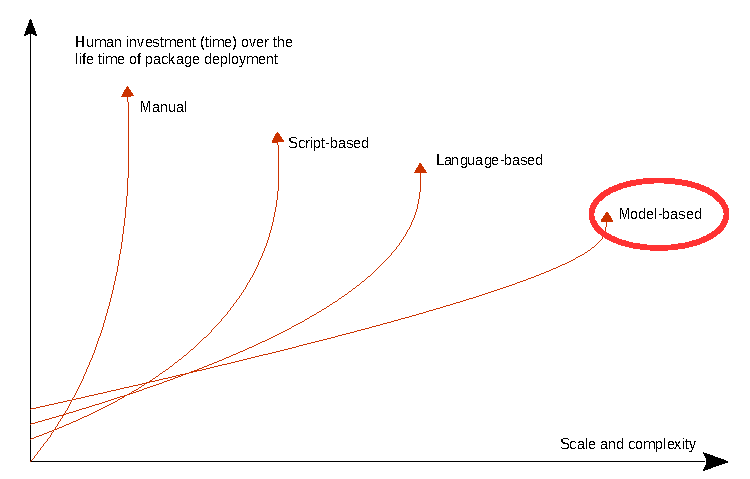
\includegraphics[width=1\columnwidth]{chapters/stateOfTheArt.images/TradeoffsDeployment.pdf}
	\caption{Tradeoffs between distributed deployment approaches (from \cite{talwar2005approaches})}
	\label{fig:tradeoffsDeployment}
\end{figure}

Thus far, the proposed deployment concept was explained, which can be represented in figure \ref{fig:DeployActivities}, including the creation, distribution and maintenance of a given application.
This process can be valid for any application, for both classical distributed and IoT systems.
However, there is no a clear nor standard way to develop applications for devices being part of the IoT.
As of classical distributed systems, three categories of solutions are studied\cite{talwar2005approaches}: script based, language-based and model-based deployment.
The trade-offs presented in this article for these different approaches are shown in figure \ref{fig:tradeoffsDeployment}.
As depicted, required time to establish a language-based and model-based approaches is clearly higher than manual and script-based, but can scale easily and handle deployment of complex systems.
\begin{itemize}
	\item \textbf{Scripted Deployment.} With the aid of scripts (i.e. bash scripts), existing tools are coordinated for conducting common deployment activities on distributed environments.
	Remote request for files using tools such as scp over ssh are often used to copy files, described in configuration files.
	Execution of package managers to install software packages is also commonly used.
	
	Usually system administrators are familiar with these tools, thus it can be very convenient at first glance, as a fairly straightforward and fully customizable approach.
	On the other hand, it can be complicated to maintain, and very time consuming when more complex use-cases are targeted.
	Moreover, models of products and site are often limited to ad-hoc models or simply inexistent.
	In order to achieve automation it can be necessary a high level of expressiveness for resource description, which is also limited in this approach.
	One of the biggest problems using this method is the lack of traceability while leaving system administrators to enact deployment via scripts.
	Indeed, human errors are more susceptible to appear since it is not possible to simulate or verify the script before running, which can result in a downtime of the distributed system.
	
	\item \textbf{Language-based Deployment.} One of the improvements of script-based deployment is the use of language-based approaches.
	The deployment tasks are performed leveraging a configuration language, parsers and other tools.
	Deployers such as SmartFrog\cite{goldsack2003smartfrog} and the one proposed in  \cite{wang2006language} are examples of the utility of this approach.
	Specialized deployment languages offer an easier usage of these tools.
	Nevertheless, execution of this method and scripted deployment are very similar, apart from the specialized language.
	
	A management runtime is often included with this language-based deployment frameworks, while the deployment workflow and the system configuration are described by the proposed language.
	Moreover, an abstraction layer is also defined for managing the configurations of deployed software. 
	Indeed, a dedicated agent can then coordinate the deployment tasks according to the provided workflow, which is then executed by the distributed deployment engine achieving the maintenance of a desired application state.
	A higher level of abstraction is then provided by this language-based approaches, describing the actions of the deployment process, in contrast with script-based approaches.
%	Software reconfiguration, automated updates and on-demand deployment are then associated to provide management strategies.
	However, language-based deployment modeling does not allow for full deployment automation.
	Indeed, association between custom automation policies seems to be difficult, even if the language facilitates it by specifying the deployment.
	Moreover, heterogeneity of resources and components is not well handled by the language-based approach, as the engine that executes the language should still cope with heterogeneous products and site models.
	These final issues are addressed by model-based deployment techniques.
	
	\item \textbf{Model-based Deployment.} An architectural model is used by model-based deployment for modeling structure of a software application together with the target execution environment.
	Two sides of the architectural model can be appreciated, one including components, connectors, component configurations and their requirements, while the other side targets execution nodes, network connections and resources.
	One of the key advantages of this approach is the decoupling of software and environment models.
	Moreover, the relationship between applications and the target environment are also represented.
	The requirements for composing components are declared on the software model, and target environment descriptions including features and resources are exposed by the runtime model.
	A high automation level of the process is achieved by using these models, while the reusability is improved.
	When the software is deployed in different execution environments, the re-usability of the model is very useful.
	In the same way, the model of the execution environment may be reused for deployment of many different applications. 
	Based on the architectural model created during the development phase, component-based systems are helpful to define the software deployment model.
	Thus, model-based approaches and component-based approaches are specially suitable to conceive an automated tool for distributed software deployment.
\end{itemize}

As we can appreciate, even if the initial cost as well as in time as in resources can be very high, the use of model-based approaches provides better handling of a distributed system.
Thus, exploration of these methods is of high interest, since deployment on IoT systems must be managed in a very fine manner.
The next sections aim to provide a good understanding of model-based approaches.

%\subsection{Service-Oriented Components (SOC)}
%As stated in the CBSE definition, decoupling software in pieces defining roles and interfaces reduces complexity, and allows the construction of compatible implementations.
%However, in a high-level point of view, constructing applications leads to make a choice between several implementations, and not the needed functionalities.
%Thus, a strong coupling exists between code and a given implementation.
%In a service-oriented approach, this coupling is avoided delegating the searching and instantiation of a required functionality to a central entity.
%Indeed, service-oriented components are the composition between Service-Oriented Architecture (SOA) and component models, which results in high decoupling and increased flexibility.

%The general principles of a Service-Oriented Component Model were described by Cervantes \textit{et al.}\cite{cervantes2004autonomous}, seen as a SOA extension to component based development.
%These principles are:
%\begin{itemize}
%	\item \textbf{A service is a provided functionality.} A service is a set of reusable operations.
%	\item \textbf{A service is described by a service specification.} It can contain syntactical, behavioral and semantic informations, as well as other specification dependencies.
%	\item \textbf{Components implement service specifications.} Being the services the only way of communication between component instances, constraints given by these specifications must be respected.
%	\item \textbf{The interaction mechanisms of the service approach are used to solve dependencies between components.} The services, provided by the component instances, are stored in a service registry. This registry is then used to dynamically discover services in order to solve dependencies between them.
%	\item \textbf{Compositions are described using services' specifications.} An abstract composition is an specification of services which allows the selection of concrete components. The links are inferred from the services' dependencies.
%	\item \textbf{Service specifications provide the basis for substitutability.} A component can be replaced by another having the same specification.
%\end{itemize}

%Unlike traditional component models, in which we select components before runtime, the interaction principles of the services approach allows to delay this selection until runtime (i.e. from a service provider).
%The application will start only if all dependencies of the main component are satisfied.
%Another main difference is that the application is defined in a higher abstraction level, in terms of service specifications and not in terms of implementations.
%Thus, the result is a Service-Oriented component model facilitating the construction of flexible and dynamic applications.OSGi and iPOJO, two approaches leveraging the main advantages of the two concepts (loose-coupling and dynamism from the services approach, and a simple development model with a description of the composition from component models) are presented in the next subsections.

%A propos du chapitre 3 :
%Le titre devrait être : Deployment in distributed systems
%L'introduction devrait pas être du background de nouveau, car la transition doit être fait en fin de chapitre 2.
%Personnellement, je changerai l'ordre c'est pas très logique. 
%Je mettrais le CBSE en premier car cela correspond à l'approche traditionnel pour faire du déploiment en système distribué, et je pense que c'est ce qu'il faut dire au début.
%Ensuite tu parles du M@R (en le présentant comme une évolution du CBSE) et à l'intérieur tu peux parler du MDE. Mais le MDE dans l'absolu ce n'est pas important pour toi. etc...


\subsection{Model-based engineering tools for software deployment}
With a view to ease software development and deployment for these very complex information systems, Model Driven Engineering (MDE) focus on, at first, giving simple, abstract and different points of view of information systems, without modify the actual system. 
In a second place, a variant of the MDE approach, called Model Driven Architecture (MDA)\cite{kleppe2003mda} aims to provide, through Domain Specific Languages (DSLs) coupled with code generators, software development tools and methods.
This approach is able to generate executable code from the abstract model, that can be generated for different hardware architectures.
Moreover, while heterogeneity of target architectures is taken into account through multiple generators, they also imposes a V cycle of development\cite{fouquet2013kevoree}, which consists in:
\begin{itemize}
	\item Context design of the abstract system ("Meta-model" and code generators)
	\item Use-case design (model)
	\item Executable code from the model
\end{itemize}
Even if this V cycle responds to the large complexity, it could not be enough to respond in terms of software plasticity that will be present in the very changing IoT environment.

We can consider this critical systems as \textit{Dynamic Adaptive Systems} (DAS)\cite{mckinley2004composing}, \cite{morin2009taming}.
Continuous update mechanisms are then carried into the target platforms, in order to change at runtime the software already deployed.
Taking into account this dynamic behavior, DAS are defined using a paradigm based on components, being the management of these components' deployment an evolution of the approach. %which allows to decouple this big systems into software pieces that are easily maintainable\cite{crnkovic2002building}.

DAS were typically deployed on critical platforms such as airports or banks, which had no tolerance to downtimes.
However, in the last years the pervasiveness of software in all domains demand a downtime rate near to zero, including phones, domestic Internet gateways and domotic services\cite{nain2008using}.
This requirements need to be supported by continuous updates, even for this non-critical systems.
Even if today IoT systems are not widely deployed, its importance in the near future justify its design in the form of a DAS.

The development model was also changed drastically, in order to follow the software plasticity present in this systems.
When V cycle was widely used and preferred over other development methods in the 80's, coming from the design and initial specification to the code generation or implementation, nowadays Agile methods\cite{stolberg2009enabling}, which aim to bring in shorter development cycles, are more recommended and used, in order to respond more quickly to specification evolutions thanks to users feedback.
Combined to this, the new approach of Continuous Integration (CI) introduces a new test system able to be updated with new artifacts of continuous development.
By adopting such a methodology, non-critical systems and DAS specified constraints are brought more closely, supporting the idea of move together abstractions of this two domains.

Therefore, the V approach from the 80's is becoming obsolete, while agile methods tend to expand it at every development cycle.
It is then possible to develop and deploy software for critical and non-critical systems in a continuous manner.
MDE approaches to generate code, and especially the MDA unidirectional approach which leverages a model to produce code, must take into account the inherent bidirectional development model of this continuous cycle.
Moreover, generators must provide reverse operations to allow cyclic code, which can be present at design time.
This can be useful to deal with legacy code as much as at design time, which is one of the main concerns of MDE, as in the tooling, beyond an approach of \textit{design-to-code}.

\subsection{M@R in Dynamic Adaptive Systems (DAS)}
\begin{figure}[]
	\centering
	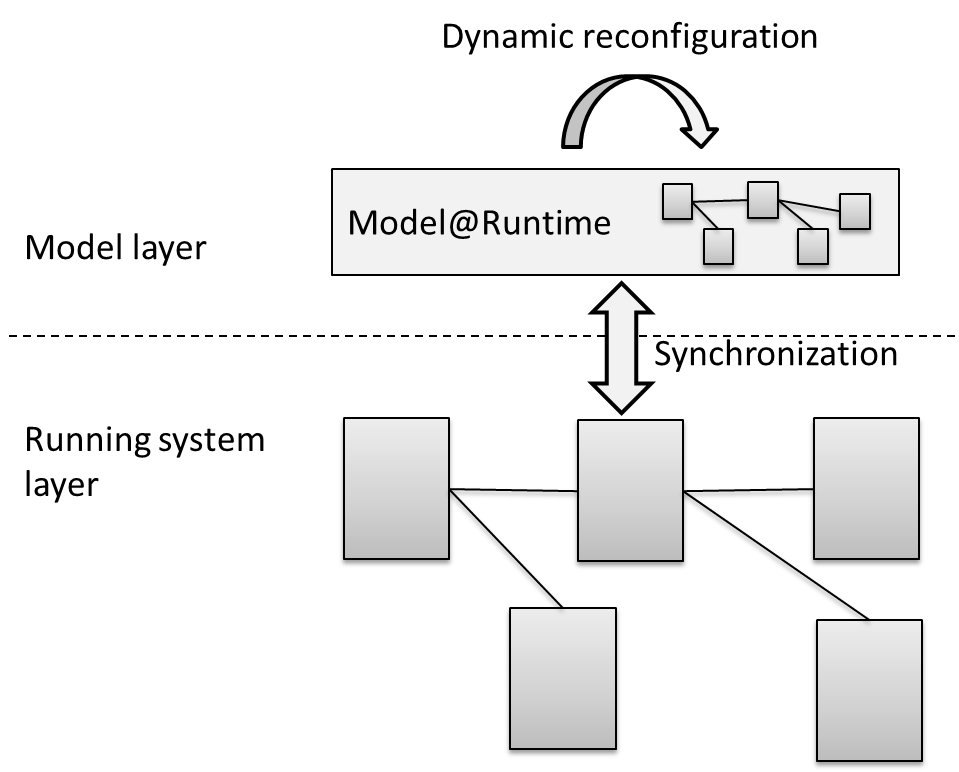
\includegraphics[width=0.65\columnwidth]{chapters/stateOfTheArt.images/MAR_Overview.png}
	\caption{Model@runtime principle} 
	\label{fig:MAROverview}
\end{figure}
A paradigm named \textit{Model@Runtime} (M@R) aim to combine MDE techniques with tangible systems, in order to respond to the problem of cyclic design stated previously.
As MDE, M@R were useful at first as a thoughtful visualization of a system, for simulation purposes\cite{oreizy1999architecture}, \cite{blair2009models}, \cite{zhang2006model}.
A \textit{permanent updated} model is then used to represent abstractly a DAS at runtime.
Every different element composing this model can be represented in a schema, providing an easy navigation and an introspective analysis through the model layer.
Reasoning about the state of the system is also possible using the same layer.
Leveraging not only the introspection capability of the model, but also the intersection, Brice Morin\cite{morin2010leveraging} worked with this Model@Runtime layer aiming to modify it, through the reflexive model representation.
Using intersection allows to modify the internal state of a system\cite{paepcke1993object}.
Morin's M@R approach aim to build systems with reflexive capacities, having also intersection and introspection features present in the same layer.
As an abstract layer, the proposed reflexivity can be asynchronous, allowing modifications before affecting the real system, i.e. for testing purposes. 
The principle of model@runtime is illustrated on figure \ref{fig:MAROverview}.

This asynchronous properties separate strongly the actual system and the model, giving to MDE techniques the possibility to manipulate the reflexive layer without affecting at all the running platform.
Moreover, a schematic representation leveraging the reflexive layer can be extracted from the actual system, in order to modify it.
This modification can be in the form of component's adding or removal in the extracted model, then thanks to a version comparison between both the actual and the modified model, it is possible to actually trigger updates on the platform.
A bidirectional connexion also exists, since any modification to the external platform will be reflected in the M@R layer.
Modifications in the model can be manipulated before the deployment allowing verifications, in addition to a more flexible way to test different configurations.
For instance, if we want to deploy components with dependencies, the platform itself will avoid the deployment if any of the dependencies are not met.
At the model level, the same changes can be executed regardless of the order, if the adaptation execution is done after the adding/removal of the components, being the model less constrained than the platform.
While the restrictions of the platform avoid the direct use of MDE approaches to manage the adaptations, the model can be manipulated to delay this restrictions in the application of the reflexive model, allowing to MDE approaches manipulate the model without following any order.

Approaches such as feature models or aspects\cite{morin2009taming} coupled with composition algorithms, can leverage the asynchronous capabilities of M@R in order to compose a model from the DAS architecture.
Since all operations can be done \textit{offline}, no constraints are imposed by the tangible platform before the deployment, while the system can decide when to synchronize.
Conceiving and composing models is then essential to assemble a whole DAS.
Indeed, several paradigms of composition are also needed, based in previous works\cite{morin2009mar},\cite{ko2012low},\cite{rouvoy2009music}, that encourage the use of software components to encapsulate the life cycle and composition operators.
Moreover, this paradigms are also needed to explore the exploitation viability at this granularity level, in order to manage the different parts of DAS application layer. 

%An IoT system is very complex and should be implemented as a DAS.
%This is important because the management of IoT infrastructures is impossible if the current approaches still being used, since each subsystem is treated as a separated entity of the whole system.
%The limitations given by the hardware of IoT devices must be taken into account, while providing the means to reach an abstraction level typical of DAS design.
%The very hard task to decouple an embedded application into small pieces should be coped using a CBSE approach, since works converge in the use of this method for DAS

%\subsection{Special distributed systems: Wireless Sensor Networks}

\subsection{Kevoree}
\label{subec:kevoree}
The Kevoree\footnote{\url{http://www.kevoree.org}} project, was created as a part of Fran{\c{c}}ois Fouquet's PhD thesis.
A part of the contributions of this thesis were based on this project, being the most important the implementation of the Kevoree meta-model in C language and the adaptation of an essential part of the framework as a Contiki OS\cite{dunkels2004contiki} application for the IoT.
This section presents the most important concepts that were essential to the achievement of this thesis.
This concepts are thus very important to the general understanding of the next chapters.

Kevoree is a component-based development framework for applications running on DAS, based on the paradigm of Models@Runtime.
This approach proposes an abstract model through which it is possible to manipulate the different concepts that characterizes a distributed system.
It provides the following concepts to design a distributed system featuring dynamic adpatations:
\begin{itemize}
	\item \textbf{The Node concept} is used to model the infrastructure topology.
	\item \textbf{The Group concept} is used to model the semantics of inter-node communication, particularly when synchronizing the reflection model among nodes.
	\item \textbf{A Channel concept} is included in Kevoree to allow for different communication semantics between remote Components deployed on heterogeneous nodes. 
\end{itemize}
All Kevoree concepts \textit{(Component, Channel, Node, Group)} obey the object type design pattern\cite{woolf1996type} in order to separate deployment artifacts from running artifacts.

\subsubsection{Main Kevoree features}
Kevoree aims to provide an abstraction able to manipulate the main concepts of a distributed system, in order to ease the adaptations management for this system.
To do that, Kevoree proposes several features: synchronization and de-synchronization between the reflexive model and the actual system at runtime, separation of concerns between the business logic and its interactions and finally the dissemination of reconfigurations and resource heterogeneity on which the system is being executed.
\begin{description}
	\item [Separation of concerns.] A distributed application is composed of specific business logic but also communication means (code).
	Unlike business logic, communication means does not have necessarily specific code due to the application.
	Thus, it results interesting to separate these two entities, which allows to reuse the different software blocks.
	This simplifies the component's business logic development, since the communication concerns are separated thus hidden.
	Moreover, the adaptation of the communication means between components regarding the context is required for a distributed application.
	\item [Distribution management.] In order to distribute different functionalities to the different nodes in a system, an abstract representation is provided, in which this characteristics are modeled and can be manipulated at runtime.
	\item [De-synchronization.] A process of validation carried in the reflexive model before the application is one of the main advantages of this feature.
	This de-synchronization is possible thanks to the concept of models@runtime that is the base of Kevoree, in which an adaptation is defined through a model that can be validated.
	Coherence of the configurations is then validated to be sure that an unstable behavior can be reached or a complete breakdown can happen.
	In a distributed context, this is of high importance, in order to avoid an adaptation that cannot be executed by all nodes.
	\item [Adaptations dissemination.] Once an adaptation is executed, every node must be notified of this change, so it can be taken into account by the whole system.
	However, in a distributed system, and specially in an IoT system, it is not possible to guarantee an uninterrupted communication between nodes, since IoT networks are often a subject of communication errors or disconnections.
	This constraints are considered in the dissemination of the adaptations, to provide a coherent evolution.
	Different synchronization methods are then used regarding the communication means between nodes.
	\item [Execution platforms heterogeneity.] Distributed systems are composed of several execution platforms, such as mobile nodes (smartphones), PC, servers or embedded systems. In the particular case of the IoT all this kind of systems are involved, since the tasks are distributed according to the hardware capacities of the available platforms.
	It is then necessary to represent in the Kevoree model the differences between participants and their specific characteristics.
\end{description}

%\subsection{Kevoree internals}
Kevoree supports multiple execution platforms (e.g., Java, Android, MiniCloud, FreeBSD, Arduino).
For each target platform it provides a specific runtime container.
As a result, Kevoree offers an environment to facilitate the implementation of dynamically reconfigurable applications in the context of distributed systems. %

\subsection{A DAS for the IoT: Challenges}
Given the complexity and the vast heterogeneity of an IoT architecture, this thesis proposes the use of a M@R approach to manage the life cycle of the software deployed in this systems.
The approach will follow the directions given by the research already done by Fran{\c{c}}ois Fouquet\cite{fouquet2013kevoree}, previously based on Brice Morin's thesis\cite{morin2010leveraging}.
The DAS representation of the IoT will result, as in the mentioned thesis, in a Dynamic DAS (DDAS), in which we found a very different behavior than in traditional DDAS, such as Data Centers or Cloud Computing.
The challenges raised by such an approach in an IoT environment are, first of all, linked to the constrained environment already described in section \ref{subsec:constrainedObj}.
As the current implementations of the M@R paradigm are done in high level languages, one main challenge is to adapt such implementations to development environments for embedded systems in which we cannot make use of such high-level languages, resulting in a difficult development task.
Moreover, the decoupling of components in modern operating systems is facilitated by Inter Process Communication (IPC) APIs already provided.
In the OS described in section \ref{subsec:IoTOS}, and more particularly in Contiki, IPC are less evident nor standard.
Thus, a new way to implement components must be proposed following the directions discussed in section \ref{sec:CBSE}.
A second challenge resides in the network topology typical of IoT.
Being a multi-hop communication the mainly used approach to reach nodes in the IoT, different abstractions are needed to take it into account.
Furthermore, the network traffic must be reduced to a minimum, since wireless devices use batteries to work, and being communication the most energy consuming task of an IoT node.

\section{Dynamic deployment in the IoT}
\label{sec:IoTDeployment}
The process of software deployment can differ significantly from classical distributed systems to IoT systems.
This is due to the underlying hardware differences discussed throughout this state of the art.
While non-constrained nodes present in classical distributed systems are able to run VMs to execute precompiled bytecode, written in high level languages such as Java, IoT devices are not able to run a complete JVM, but rather very limited ones\cite{levis2002mate}\cite{brouwers2009darjeeling}.
Moreover, related research\cite{oliver2014reprogramming} found JVMs very resource consuming in small devices typical of IoT, since they add a considerable CPU overhead while running, which avoids a long-term use for battery powered nodes.
Thus, we will focus on software deployment for applications compiled as binary code, which can be executed directly by the native platform.
Indeed, in the embedded systems domain, which embodies most of the devices used in IoT, bare metal applications are the most common procedure to provide services or functionalities.
Physical flashing of the binary image is the usual deployment method, since it can be done at the manufacturing step of the embedded system, without considering any further firmware changes.
With this limitation, it is even more complicated to distribute applications among several nodes which are physically separated, since manual flashing of every node in a typical IoT system cannot be worth considering due to the huge amount of nodes.
Thus, a choice of the current alternatives to deal with this problem should be made.

Operating systems used in embedded systems and Wireless Sensor Networks (WSN) provide several methods to deploy new applications at runtime, being the most common:
\begin{enumerate}
	\item Scripting languages \cite{dunkels2006low}\cite{kovatsch2012actinium}.
	\item Virtual Machines.
	\item Kernel replacement.
	\item Position Independent Code.
	\item Relocatable code.
\end{enumerate}
As we discussed in this section, research shows that only non-interpreted code is worth considering for long term applications.
Thus scripting languages and VM approaches will be discarded as a method to deploy new features, in the context of this thesis.

As presented in this section, applications deployment for IoT systems differs in several ways from classical distributed systems.
In order to cope with this differences, which are mostly hardware and network related, approaches coming from the embedded systems and WSN domains have been proposed.
We will discuss three methods already introduced above: 
\begin{itemize}
	\item \textbf{Kernel replacement.} This is a straightforward solution to deploy new features or bug fixes in embedded systems, an essential part of the IoT infrastructure presented in this thesis.
	It consists in change the entire kernel image for a new one, which must be either flashed physically or transmitted through the network, followed by a complete reboot of the system.
	Indeed, sharing a large kernel image can be very energy consuming for wireless battery powered devices.
	Advantages of this technique are the possibility of deep changes into the kernel or applications, as well as deployment of a complete different OS.
	\item \textbf{Position Independent Code (PIC).} As mentioned previously in this chapter, the executable code usually follows the process of dynamic relocation to find the needed symbol's addresses, then execute the code. 
	PIC follow a different approach to run applications. 
	It consists in the use of relative jumps rather than absolute addresses to find symbols, mitigating the need of run-time relocation.
	Several overheads can be introduced by the use of this technique, such as pre-loading of addresses before making jumps, more needed jumps while calling kernel or another module, functions registration and de-registration and the necessity of a jump table.
	Furthermore, a PIC compatible compiler should be used, in order to produce a loadable module using this method, which can be unavailable for certain CPU architectures.
	For instance, AVR microcontrollers supports this type of compilation, but it is limited to a 4KB program size, while it is not known a compiler supporting PIC for MSP430 CPUs.
	Applications running non-PIC methods to deploy new modules have shown a 13\% better performance compared to PIC\cite{dong2009dynamic}.
	However, the global efficiency while running most of PIC modules is the same as if they were flashed directly on the device.
	\item \textbf{Relocatable code.} This technique is the one used by classical OSs such as Unix based and Windows, also implemented for IoT devices\cite{dunkels06runtime}. 
	It uses run-time dynamic linking, relocation and loading of modules compiled using the standard Executable and Linkable Format (ELF).
	This format includes the program code and data, as well as detailed information about unresolved symbols.
	To resolve them, the OS must adjust properly the absolute addresses included in the file, depending on the module's location in memory.
	A relocation type also embedded in the ELF file specifies how the data or code addresses should be updated.
	These types depend on the CPU architecture, for instance, an MSP430 CPU counts with only one type of relocation, while the AVR architecture has 19.
	Both architectures are widely used for embedded systems and IoT devices.
	Once each unresolved symbol is updated with the new address, the \texttt{.data} and \texttt{.bss} sections of the ELF file can be loaded into RAM, and the \texttt{.text} is copied to ROM, then the program can be executed following specific OS functions.
	Overheads of this method include the transmission over the network of a large ELF file depending on the 32 or 64 bits architecture, a symbol table in which names are used to represent each unresolved symbol, also increasing the size of the ELF file, and finally a CPU overhead is incurred while resolving symbols.
	As in the PIC method, no reboot is required to run the new application or to apply an update.
\end{itemize}

\begin{table}[htb]
	\scriptsize
	\centering
	\caption{Feature Comparison (adapted from \cite{oliver2014reprogramming})}
	\label{tab:deployMethods}
	\begin{tabular}{lccccccc}
		& \multicolumn{3}{c}{\textbf{Mechanism}}       & \multicolumn{4}{c}{}                                                                                          \\
		& \textbf{VM} & \textbf{PIC} & \textbf{Reloc.} & \textbf{OS Protection} & \textbf{Kernel Modif.} & \textbf{Kernel Replacement} & \textbf{Loose Coupling} \\ \hline
		Mat\'e\cite{levis2002mate}      & $\bullet$           &              &                 & $\bullet$                      &                              &                             & $\bullet$                      \\ \hline
		TOSBoot\cite{hui2004dynamic}    &             &              &                 &                        &                              & $\bullet$                           &                         \\ \hline
		SOS\cite{han2005dynamic}        &             & $\bullet$            &                 &                        & $\bullet$                            &                             & $\bullet$                       \\ \hline
		Contiki\cite{dunkels2004contiki}    &             &              & $\bullet$               &                        &                              & $\bullet$                           & $\bullet$                       \\ \hline
		RETOS\cite{cha2007retos}      &             &              & $\bullet$               & $\bullet$                      & $\bullet$                            &                             & $\bullet$                       \\ \hline
		Darjeeling\cite{brouwers2009darjeeling} & $\bullet$           &              &                 & $\bullet$                      &                              &                             & $\bullet$                       \\ \hline
		SenSpire\cite{dong2009dynamic}   &             &              & $\bullet$               &                        & $\bullet$                            &                             & $\bullet$                       \\ \hline
		Enix\cite{chen2010enix}       &             & $\bullet$            &                 &                        &                              &                             &                         \\ \hline
	\end{tabular}
\end{table}

Other features of the proposed approaches can be considered, such as OS protection, low level kernel modification and even a whole kernel replacement.
The loose coupling between new added modules and the underlying kernel is also important, since added flexibility of development allows scalability and fast upgrade of components.
Several operating systems using the discussed approaches are shown in table \ref{tab:deployMethods}.
VMs are included in this table since they offer high loose coupling and OS protection, and can be suitable for very short life-cycle applications running on IoT devices.

%\section{Related work}
%\todo{Maybe a synthesis of the related work presented in the 2 papers is worth to consider?}


\section{Conclusion}
In conclusion, even if deployment mechanisms for IoT devices exist and can be improved to reach a good reliability level and ease to use, manual installation or updates of features should not be worth considering, as it was explained in the previous section.
Moreover, figure \ref{fig:tradeoffsDeployment} already shows that in classical distributed systems manual deployment is not suitable for large-scale systems.

Given the available methods of deployment for new applications or feature updates, it is then necessary to evaluate which is the most advisable approach for its use and adaptation in an automated deployment manager.
Taking into account the already described model-based techniques, the criterion to evaluate the previously presented approaches will be based on the capability of such approach to be easily decoupled into components, that can be disseminated over the network using a minimum of transfers.
It is very important to have a good implementation of the local deployment procedures, as well as the necessary tools to share deploy units to the rest of the nodes.
As presented in the previous chapter, the Contiki OS seems to provide the necessary tools required above.
Thus, for this thesis, the use of Contiki as the underlying platform to validate our approaches has been chosen.
This leads to a deeper understanding of the OS internals and a big effort to implement the high level abstractions required by the use of model-based deployment approaches.

The presented CBSE and Models@Runtime concepts are essential to build our IoT software architecture.
Indeed, being our goal the design and implement a software layer manager dedicated to IoT systems in order to enable automatic deployment and dynamic adaptations, the introspection and the dynamic reconfiguration facilities offered by Kevoree seems to suit our needs.
Thus, the need of an unified tool managing the software layer of the system comes with the design of such architecture.
However, at this point the main differences regarding IoT systems and classical distributed system become more relevant, since the already investigated approaches are intended for the latter.

Taking this state of the art as a source of inspiration, the purpose of this thesis is to propose a novel way to manage software deployment in IoT systems, facing at the same time the common issues of distributed systems and the new ones raised by the constraints of IoT devices.

The next chapters are intended to explain the main contributions of this thesis, leveraging the already discussed topics on this chapter to propose an automated deployment engine for IoT applications, based on the three tools already discussed in section \ref{sec:softDeployment}, in addition to the Kevoree meta-model and the Contiki OS.